\graphicspath{{graphix/}}


%----------Packages---------------
\usepackage{ragged2e}\justifying
\usepackage{txfonts}
\usepackage{graphicx}
\usepackage{fontawesome}
\usepackage{pifont}
\usepackage{tikz}
\usepackage{totcount}
\usepackage{refcount}
\usetikzlibrary{patterns.meta}
\usetikzlibrary{fadings,patterns,shadows}
\usepackage[nodayofweek]{datetime}
\usepackage{comment}
%-----------------------------------

%--------theme settings------------
\usetheme{Madrid}
\useoutertheme[subsection=false]{miniframes}
\setbeamertemplate{navigation symbols}{}
%\setbeamertemplate{itemize item}{\bfseries\ding{228}}
\setbeamertemplate{itemize item}{%
	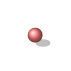
\begin{tikzpicture}
		\shade[ball color=red!50!white, preaction={fill=black,
			opacity=.25,transform canvas={xshift=1mm,yshift=-1mm, yscale=0.5}}] (0,0) circle (0.6ex);
	\end{tikzpicture}
}
\setbeamertemplate{frametitle}[default][left, leftskip=2mm] 
\setbeamertemplate{footline}{
	\leavevmode\bfseries 	
	\begin{beamercolorbox}[wd=0.3\paperwidth, ht=7pt, dp=2.5pt, center]{author in head/foot}
		\insertshortauthor~\insertshortinstitute
	\end{beamercolorbox}%
	\begin{beamercolorbox}[wd=0.38\paperwidth, ht=7pt, dp=2.5pt, center]{title in head/foot}
		\insertshorttitle
	\end{beamercolorbox}%
	\begin{beamercolorbox}[wd=0.22\paperwidth, ht=7pt, dp=2.5pt, center]{date in head/foot}
		\insertshortdate
	\end{beamercolorbox}%
	\begin{beamercolorbox}[wd=0.1\paperwidth, ht=7pt, dp=2.5pt, center]{page number in head/foot}
		\insertframenumber/\inserttotalframenumber
	\end{beamercolorbox}%
}
\setbeamertemplate{enumerate item}{\bfseries(\arabic{enumi})}
\setbeamertemplate{enumerate subitem}{\bfseries(\alph{enumii})}
\begin{comment}
	\setbeamertemplate{headline}{
	\leavevmode\bfseries 	
	\begin{beamercolorbox}[wd=0.25\paperwidth, ht=7pt, dp=2.5pt, center]{section in head/foot}
	\insertsectionhead 
	\end{beamercolorbox}%
	\begin{beamercolorbox}[wd=0.75\paperwidth, ht=7pt, dp=2.5pt, center]{palette quaternary}
	\insertsectionnavigationhorizontal{0.75\paperwidth}{\hfill}{\hfill}
	\end{beamercolorbox}%
	}...
\end{comment}




%\setbeamertemplate{background canvas}{
%	\includegraphics[width=\paperwidth, height=\paperheight]{bg}
%}
%-------------------------------------

%-----Font Settings---------------------------
\usefonttheme{serif}
%\usepackage{fontspec}
\setbeamerfont{section in head/foot}{series=\bfseries}
\setbeamerfont{title}{series=\bfseries,size=\Large}
\setbeamerfont{date}{size=\scriptsize}
%\setmainfont{Georgia} 
%\setsansfont{Trebuchet MS} 
%\setmonofont{Inconsolata}

%---------colour definitions-----------

\definecolor{denim}{rgb}{0.08, 0.38, 0.74}
\definecolor{cadmiumgreen}{rgb}{0.0, 0.42, 0.24}
\definecolor{carolinablue}{rgb}{0.6, 0.73, 0.89}
\definecolor{cerulean}{rgb}{0.0, 0.48, 0.65}
\definecolor{anti-flashwhite}{rgb}{0.95, 0.95, 0.96}
\definecolor{blue-violet}{rgb}{0.54, 0.17, 0.89}
\definecolor{magnolia}{rgb}{0.97, 0.96, 1.0}
\definecolor{flame}{rgb}{0.89, 0.35, 0.13}
\definecolor{deeppeach}{rgb}{1.0, 0.8, 0.64}
\definecolor{cadet}{rgb}{0.33, 0.41, 0.47}
\definecolor{ceil}{rgb}{0.57, 0.63, 0.81}
\definecolor{darktaupe}{rgb}{0.28, 0.24, 0.2}
\definecolor{arsenic}{rgb}{0.23, 0.27, 0.29}
\definecolor{cornflowerblue}{rgb}{0.39, 0.58, 0.93}
\definecolor{hooker\'sgreen}{rgb}{0.0, 0.44, 0.0}
\definecolor{gainsboro}{rgb}{0.86, 0.86, 0.86}
\definecolor{isabelline}{rgb}{0.96, 0.94, 0.93}
\definecolor{myYellow}{HTML}{ee9b00}
\definecolor{mySeaGreen}{HTML}{e0fbfc}
%-------------------------------------

%-------------Colour Settings
\setbeamercolor{title}{bg=denim,fg=anti-flashwhite}
\setbeamercolor{itemize item}{fg=flame}
\setbeamercolor{enumerate item}{fg=red}
\setbeamercolor{title in head/foot}{bg=white,fg=cadmiumgreen}
\setbeamercolor{author in head/foot}{bg=white,fg=cadmiumgreen}
%\setbeamercolor{section in head/foot}{bg=magnolia,fg=blue-violet}
\setbeamercolor{frametitle}{bg=white,fg=cerulean}
\setbeamercolor{date in head/foot}{bg=white,fg=cadmiumgreen}
\setbeamercolor{page number in head/foot}{bg=white,fg=cadmiumgreen}
%\setbeamercolor{progress bar}{fg=green,bg=blue}
\setbeamercolor{section in head/foot}{fg=hooker\'sgreen,bg=anti-flashwhite}
\setbeamercolor{palette quaternary}{bg=gainsboro}
%-----------------------------------------------------------

%---------Other-----------------
\longdate
%---------------------------------------


%--------Progress BAR-----------
\setbeamercolor{progress bar progress}{use=progress bar,bg=progress bar.fg}
\defbeamertemplate{footline}{progress bar}{
	\dimen0=\paperwidth
	\multiply\dimen0 by \insertframenumber
	\divide\dimen0 by \inserttotalframenumber
	\edef\progressbarwidth{\the\dimen0}
	
	\leavevmode%
	\begin{beamercolorbox}[wd=\paperwidth,ht=0.1ex,dp=1ex]{progress bar}
		\begin{beamercolorbox}[wd=\progressbarwidth,ht=0.1ex,dp=1ex]{progress bar progress}
		\end{beamercolorbox}%
	\end{beamercolorbox}%
}

\setbeamertemplate{footline}[progress bar]
\setbeamercolor{progress bar}{fg=myYellow,bg=mySeaGreen}

%------------------------------------------------------------------------



